
\documentclass[11pt, oneside]{article} 
\usepackage{amsmath, amsthm, amssymb, wasysym, verbatim, bbm, color, geometry}
\usepackage{amsfonts}
\usepackage{csquotes}
% \usepackage{polski}
\usepackage[english]{babel}
\usepackage[nottoc]{tocbibind}
\usepackage{caption}
\usepackage{subcaption}
\usepackage{float}
\usepackage{graphicx}
\usepackage{circuitikz}
\usepackage{listings}


\definecolor{codegreen}{rgb}{0,0.6,0}
\definecolor{codegray}{rgb}{0.5,0.5,0.5}
\definecolor{codepurple}{rgb}{0.58,0,0.82}
\definecolor{backcolour}{rgb}{0.95,0.95,0.92}

\lstdefinestyle{mystyle}{
    backgroundcolor=\color{backcolour},   
    commentstyle=\color{codegreen},
    keywordstyle=\color{magenta},
    numberstyle=\tiny\color{codegray},
    stringstyle=\color{codepurple},
    basicstyle=\ttfamily\footnotesize,
    breakatwhitespace=false,         
    breaklines=true,                 
    captionpos=b,                    
    keepspaces=true,                 
    numbers=left,                    
    numbersep=5pt,                  
    showspaces=false,                
    showstringspaces=false,
    showtabs=false,                  
    tabsize=2
}
\lstset{style=mystyle}

% \ctikzset{current arrow scale=1.5} 
\usepackage{hyperref} % Loads the hyperref package for hyperlinks
\usepackage{enumitem}
\usepackage{tikz}
\usepackage{pgfplots}
\usepackage[T1]{fontenc}
\usepackage{algorithm}
\usepackage{algpseudocode}
\usepackage{amsfonts}
\usepackage{mathbbol}

\catcode`_=\active
\def_#1{\sb{\mathrm{#1}}}


\pgfplotsset{compat=1.18} % Set the compatibility level for pg
\usetikzlibrary{shapes.geometric, arrows, positioning, fit, backgrounds}

\hypersetup{
    colorlinks=true,
    linkcolor=blue,
    citecolor=cyan,
    urlcolor=blue!60,
    breaklinks=true,
}





\newcommand{\workSource}[2]{Text available at: \href{#1}{#2}}



\DeclareMathSizes{12}{12}{10}{8}
\makeatletter
\renewcommand\normalsize{%
\@setfontsize\normalsize{12pt}{13.5pt}% Will look incredibly crabbed if line height is too small
\abovedisplayskip 10\p@ \@plus2\p@ \@minus5\p@%
\abovedisplayshortskip \z@ \@plus2\p@%
\belowdisplayshortskip 5\p@ \@plus2\p@ \@minus3\p@%
\belowdisplayskip \abovedisplayskip%
\let\@listi\@listI%
}
\normalsize  
\makeatother

\newcommand{\der}{{\rm d}}
\newcommand{\R}{\mathcal{R}}
\newcommand{\C}{\mathcal{C}}
\newcommand{\M}{\mathcal{M}}
\newcommand{\G}{\mathcal{G}}
\newcommand{\Ron}{R_{\rm ON}}
\newcommand{\Roff}{R_{\rm OFF}}
\newcommand{\von}{V_{\rm ON}}
\newcommand{\voff}{V_{\rm OFF}}
\newcommand{\q}{q}
\newcommand{\ua}{v}
\newcommand{\ia}{i}
\newcommand{\phia}{\varphi}
\newcommand{\xw}{x}
\newcommand{\dert}[1]{\frac{{\rm d} {#1}}{{\rm d} t} }
\newcommand{\inv}[1]{\frac{1}{#1} }
\newcommand{\equal}{=}


\usepackage[style=numeric, 
            backend=biber,
           ]{biblatex}
           
\addbibresource{bibliography.bib} % Replace with your .bib file name

\geometry{tmargin=.75in, bmargin=.75in, lmargin=.75in, rmargin = .75in}  

% \usepackage{fontspec}
% \setmainfont[]{Palatino}

\newcommand{\Cdot}{\boldsymbol{\cdot}}

\newtheorem{thm}{Theorem}
\newtheorem{defn}{Definition}
\newtheorem{conv}{Convention}
\newtheorem{rem}{Remark}
\newtheorem{lem}{Lemma}
\newtheorem{cor}{Corollary}


\title{Reservoir computing}
\author{Karol Bednarz}
% \date{Rok akademicki 2024--2025}
\date{\today}

\begin{document}

\maketitle
\tableofcontents

\vspace{.25in}

\newcommand{\Todo}[1]{\textcolor                {red}{\textbf{TODO:} #1}}

\section{ESN - Echo State Network}


\subsection{Principles of reservoir computing}
Based on the~\cite{Bai2023}:
The state of reservoir dynamics can be expressed as:
\begin{equation}
    h_t = f \big((1-k) \cdot u_t \cdot W_{in} + k\cdot h_{\mathrm{t-1}} \cdot W_h + y_{\mathrm{t-1}} \cdot W_{1b} + b \big)
\end{equation}
Where:
\begin{itemize}[noitemsep, leftmargin=4cm, label={}]
    \item [\(h_{t-1}\)] -- are the reservoir state respectively, from the previous time step,
    \item [\(u_t\)] -- is the observed data at time step \(t\),
    \item [\(y_{t-1}\)] -- is the the predicted output state \(t-1\),
    \item [\(W_{in} \in \mathbb{R}^{N_u \times N_h}\)] -- is the input weight matrix,
    \item [\(W_h \in \mathbb{R}^{N_h \times N_h}\)] -- is the internal weight matrix,
    \item [\(W_{1b} \in \mathbb{R}^{N_h \times N_y}\)] -- is the output fedback weight matrix,
    \item [\(b \in \mathbb{R}^{N_h}\)] -- is the bias vector.
    \item [\(f\)] -- is the activation function, typically \(\tanh\) or \(\mathrm{sigmoid}\),
    \item [\(k\)] -- is the leaking rate, typically \(k \in [0.1, 0.3]\).
\end{itemize}


With the computed reservoir dynamics, the output can be then obtained by:
\begin{equation}
    y_t = h_t \cdot W_{\mathrm{out}}
\end{equation}
Where:
\begin{itemize}[noitemsep, leftmargin=4cm, label={}]
    \item [\(W_{\mathrm{out}} \in \mathbb{R}^{N_h \times N_y}\)] -- is the output weight matrix.
\end{itemize}

\subsection{Echo state property}

Any system that changes in a nonlinear way can work as the reservoir. However, starting a nonlinear system with random connection strengths creates problems.
The reservoir is a system that feeds its outputs back into itself. This can make it unstable if the connection strengths aren't set up correctly. For example, if the internal connections are too strong, the system might get stuck giving the same output regardless of what input it receives. The random connection strengths must be chosen so the system doesn't grow out of control.
For the system to work well, it must follow something called the "echo state property." This rule ensures that the reservoir's behavior eventually depends on the input signal rather than just its starting conditions.
To meet this requirement, the internal connection matrix \(W_h\) is first set up using random values between -1 and 1. This matrix is then adjusted one time according to the echo state property rule:

\begin{align}
    W'_h          & = \alpha \odot {W_h}                                             \\
    W_h^{\dagger} & = \frac{\rho  W_h}{\left\lvert \lambda_{max}(W_h) \right\rvert }
\end{align}
Where:
\begin{itemize}[noitemsep, leftmargin=4cm, label={}]
    \item [\(\rho \in (0,1)\)] -- is the spectral radius, typically \(\rho \in [0.9, 1]\)
    \item [\(\lambda_{max}(W_h)\)] -- is the largest eigenvalue of \(W_h \).
    \item[\(\alpha \in (0,1)\)] -- is the sparsity coefficient, typically \(\alpha \in [0.1, 0.3]\).
\end{itemize}
The spectral radius is a parameter that determines the amount of nonlinear interaction of input components through time.

Due to the recursive nature of the reservoir layer,
such dynamics reflect trajectories of the past historical input—the short-term memory (known as the fading memory). As another critical property for computing the RC principle, short-term memory can be
quantitative measured by the coefficient of memory
capacity


\begin{equation}
    MC = \sum_{k=1}^{\infty} MC_k =
    \sum_{k=1}^{\infty} d^2(u_{t-k}, y_t) =  \sum_{k=1}^{\infty} \frac{\mathrm{cov}^2(u_{t-k}, y_t)}{\sigma^2(u_t) \sigma^2(y_t)}
\end{equation}

Where:
\begin{itemize}[noitemsep, leftmargin=4cm, label={}]
    \item [\(d^2(u_{t-k}, y_t)\)] -- is the square of the correlation coefficient between the output \(y_t\) and the input \(u_{t-k }\) with a delay of \(k\) time steps,
\end{itemize}

According to the Lyapunov stability analysis, a large memory capacity is needed to compute the RC principle, which can be achieved at the asymptotically stable region.


\subsection{Learning algorithm}
The training of the reservoir computing model involves adjusting only the output weights \(W_{\mathrm{out}}\). The input weights \(W_{in}\), internal weights \(W_h\), and feedback weights \(W_{1b}\) are typically initialized randomly and remain fixed during training. The training process can be summarized in the following steps:

\begin{equation}
    Y = H \cdot W_{out}
\end{equation}
Where:
\begin{itemize}[noitemsep, leftmargin=4cm, label={}]
    \item [\(Y \in \mathbb{R}^{T \times N_y}\)] -- is the matrix of target outputs for all time steps,
    \item [\(H \in \mathbb{R}^{T \times N_h}\)] -- is the matrix of reservoir states for all time steps,
    \item [\(T\)] -- is the total number of time steps.
\end{itemize}

In general, the \(W_{out}\) can be directly obtained by calculating the Moore-Penrose pseudoinverse of the reservoir states matrix H with respect to the target outputs matrix Y:

\begin{equation}
    W_{out} = Y \cdot H^{T} \cdot (H \cdot H^{T} + \eta I)^{-1}
\end{equation}
Where:
\begin{itemize}[noitemsep, leftmargin=2cm, label={}]
    \item [\(H^{T}\)] -- is the transpose of matrix H,
    \item [\(\eta\)] -- is the regularization parameter, typically \(\eta \in [10^{-6}, 10^{-2}]\),
    \item [\(I\)] -- is the identity matrix of size \(N_h \times N_h\).
\end{itemize}


\subsection{Model development}


The echo state network (ESN)  and the liquid state machine (LSM)  are the two representations of RC.  While ESN and LSM are topographically equivalent, the former adopts the actual numerical data from the input to compute the network dynamics, and the latter adopts the spiking signal to represent the spatiotemporal pattern. \textbf{The LSM can be also seen as a SNN, where the reservoir has numerous leaky integrate-and-fire (LIF) neurons interconnected with the same recursive nature as in ESN}. As the spiking event is involved, the training of LSM generally relies on the spike-timing-dependent plasticity (STDP)  and short-term plasticity (STP), among other training methods for spiking networks.


\section{Time-delayed reservoir computing}
Based on~\cite{Grigoryeva2016, Parlitz2024, Ortn2015}.

The model of reservoir can be written in the following general form:
\begin{align}
    \mathbf{r}(n) & = F\big( \gamma \mathbf{W}_{in} \mathbf{x}(n) + \beta \mathbf{W} \mathbf{r}(n-1) \big), \\
    \mathbf{y}(n) & = \mathbf{W}_{out} \mathbf{r}(n).
    \label{eq:tdrc}
\end{align}


Where:
\begin{itemize}[noitemsep, leftmargin=4cm, label={}]
    \item [\(\mathbf{r}(n) \in \mathbb{R}^N\)] -- is the reservoir state at time step \(n\),
    \item [\(\mathbf{x}(n) \in \mathbb{R}^d\)] -- is the input vector at time step \(n\),
    \item [\(\mathbf{y}(n) \in \mathbb{R}^p\)] -- is the output vector at time step \(n\),
    \item [\(\mathbf{W}_{in} \in \mathbb{R}^{N \times d}\)] -- is the input weight matrix, usually drawn from a random distribution \([-1, 1]\),
    \item [\(\mathbf{W} \in \mathbb{R}^{N \times N}\)] -- is the internal weight matrix, usually drawn from a random distribution \([-1, 1]\),
    \item [\(\mathbf{W}_{out} \in \mathbb{R}^{p \times N}\)] -- is the output weight matrix,
    \item [\(\gamma, \beta \in \mathbb{R}^+\)] -- are the input and feedback scaling parameters,
    \item [\(F: \mathbb{R}^N \to \mathbb{R}^N\)] -- is  the nonlinear activation function, typically \(\tanh\) or \(\mathrm{sigmoid}\).
\end{itemize}


In general, the time-delayed reservoir computing (TDRC) can be implemented using a single nonlinear node with delayed feedback loop instead of a large network of interconnected nodes. The delay dynamics create a high-dimensional state space that can be exploited for computation.
\section{Liquid State Machine -- Reservoir with spiking neurons}
Based on~\cite{Maass2011, Deckers2022}.

\begin{figure}
    \centering
    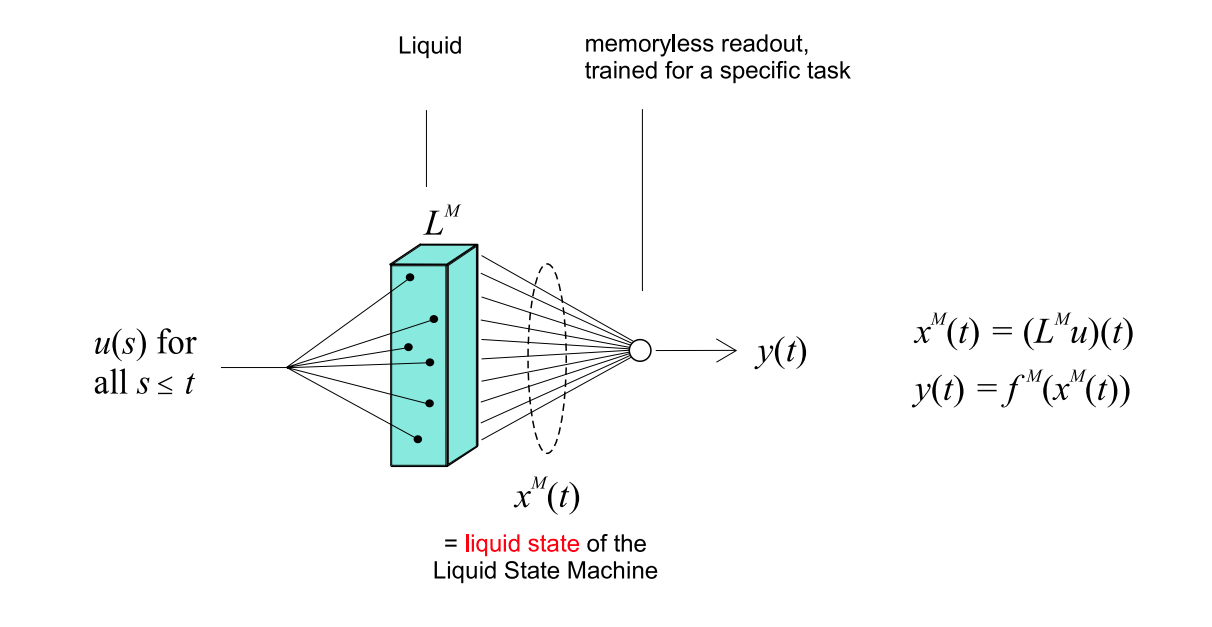
\includegraphics[width=0.8\textwidth]{figs/Liquid-state.png}
    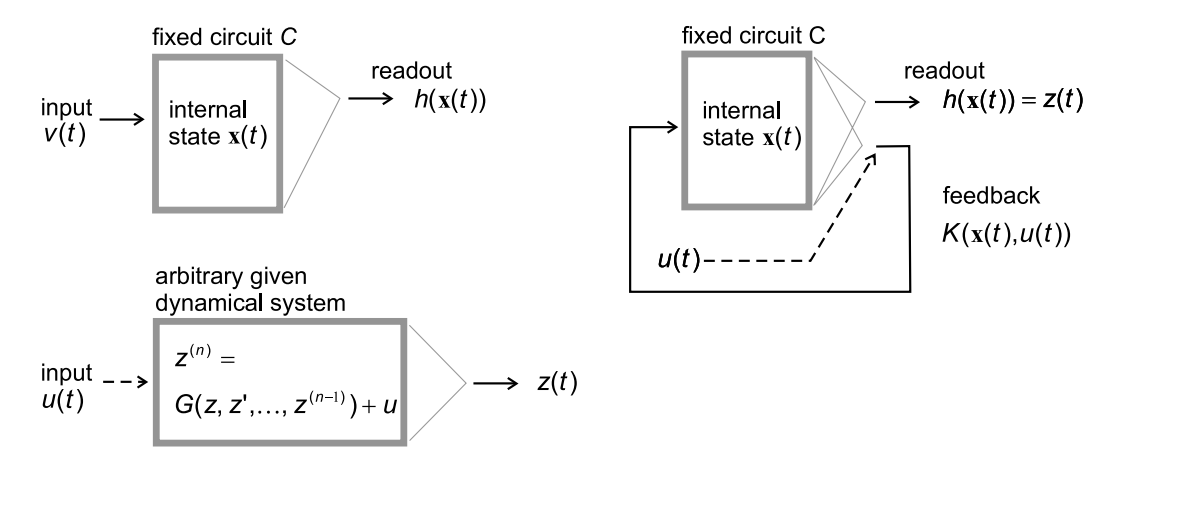
\includegraphics[width=0.8\textwidth]{figs/liquid-state-2.png}

    \caption{Liquid State Machine architecture}
    \label{fig:lsm}
\end{figure}



\clearpage
\section{Sample implementation in Python}
\printbibliography

\end{document}

